\documentclass{article}
\usepackage[utf8]{inputenc}
\usepackage[english]{babel}
\usepackage{csquotes}
\usepackage[backend=biber,style=nature,sorting=ynt]{biblatex}
\usepackage{graphicx}
\usepackage{subcaption}
\addbibresource{mybib.bib}

\title{SUHII Project Internship Report}
\author{Michael Wang}
\date{September 2019}

\begin{document}

\maketitle

\section{Objective}

The objective of this internship project was to derive the surface urban heat island intensity of cities in the TraK project by implementing the method from Li, et al. 2018 \cite{li_new_2018} on Google Earth Engine.

\section{Data and Methods}
The intensity of the surface urban heat island usually refers to the difference in land surface temperature (LST) between non-urban and urban locations.
The novelty of Li et al. 2018 \cite{li_new_2018} lies in the fact that it uses the documented relationship between LST and impervious surface areas (ISA) to fit a line between LST and ISA as a percent (\%ISA). The slope of the resulting line would have the equation:
\[f(x) = mx + b\]
\[\Downarrow\]
\[f_{LST}(\%ISA) = m(\%ISA) + ISA_{0\%}\]

Where m is the slope of the line. 

Since the intensity of the urban heat island (SUHII) can be defined as the surface temperature difference between urban and non-urban areas:

\[SUHII = f_{LST}(100) - f_{LST}(0) \]
\[\Downarrow\]
\[SUHII = (100m +  ISA_{0\%}) - (0m +  ISA_{0\%})\]
\[\Downarrow\]
\[SUHII = 100m\]

Thus SUHII is simply the slope of the fitted line multiplied by a constant of 100.
The following data was used to derive this value for each city:
\begin{itemize}
    \item A vector file of the region of interest (ROI)
    \item The World Settlement Footprint (WSF) 2015 data from DLR
    \item Landsat-derived Land Surface Temperature data from Parastatidis \cite{parastatidis_online_2017}
    \item JRC Global Surface Water Mapping Layers v1.1 from the European Commission/Google \cite{pekel_high-resolution_2016}
\end{itemize}

 The ISA data was first processed using the kernel density estimation (KDE) technique, which was applied to account for the radiance effect of impervious surfaces, where the heat of an impervious pixel is not entire contained within, as it also radiates outward into other pixels. The temperature derived from the satellite LST data, would reflect effect, thus KDE was used to account for it. The specific radius of used for the KDE will affect the results (see section 4), but a radius of 3000 meters was used in line with the original paper. Afterwards, the entire image is normalized, such that 100\% ISA refers to the most impervious areas, and 0\% the least:
 
 \[normalized = \frac{pixelvalue - minvalue}{maxvalue - minvalue}\]

The LST data is averaged at the 1km level and stacked with the max extent binary water data which was aggregated at the 1km level for a percentage. The ISA layer is then averaged at the 1km level and stacked with the other two layers. The entire stack is then clipped to the ROI, and pixels where there is more than 25\% water is removed from further analysis due to the particular thermodynamics of water.

The pixels are then grouped using the ISA layer at 2\% intervals, creating 50 "buckets" of data. This particular application did this by dividing each percentage by 2 and applying a floor function, before returning to the original range by multiplying by 2 again. For each bucket, the associated LSTs are averaged. Then a CSV with two columns is exported, with one with \%ISA at 2\% intervals, the other being the average LST for that particular interval.

The slope of the first order linear regression of these two variables would give the SUHII per the original method. For each city, the a different SUHII was derived for the summer months (May-September), winter months (October-April), and annually.

\section{Results}
The resulting files are then analyzed and visualized with python. A selection of results are shown here: 

\begin{figure}[!htb]
    \begin{subfigure}{0.333\textwidth}
        \centering
        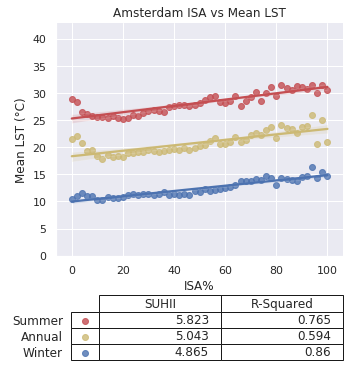
\includegraphics[width=1\linewidth]{Amsterdam3000.png}
        \caption{Amsterdam SUHII}
        \label{fig:subim1}
    \end{subfigure}\hfill
    \begin{subfigure}{0.333\textwidth}
        \centering
        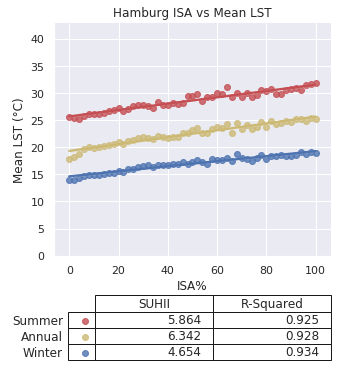
\includegraphics[width=1\linewidth]{Hamburg3000.png}
        \caption{Hamburg SUHII}
        \label{fig:subim2}
    \end{subfigure}\hfill
    \begin{subfigure}{0.333\textwidth}
        \centering
        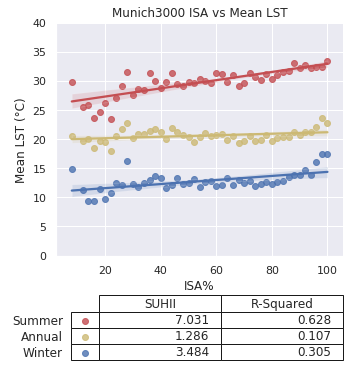
\includegraphics[width=1\linewidth]{Munich3000.png}
        \caption{Munich SUHII}
        \label{fig:subim3}
    \end{subfigure}
    \caption{A Selection of European City and the plotted \%ISA and LST}
    \label{fig:my_label}
\end{figure}

In general, the surface urban heat island effect is less intense in winter than in summer, with the annual being somewhere in the middle. The coefficient of determination ($R^2$) was also higher in summer than in winter, meaning the variances are better explained by the fitted linear regression in summer than in winter.

The SUHII value of each season for each city is appended to the original shape file as a new column through the use of geopandas.

\section{Discussion}
The $R^2$ of the fitted line varies greatly between cities, probably due to the heterogeneous and idiosyncratic nature of the urban landscape. There are a few things of note which will be elaborated on in the following sections.

\subsection{$R^2$ as a Sensitivity Test}
The authors of the original method noted the radiant effect of impervious surfaces, and applied the kernel density estimation method to avvount for it. However, this method takes one user defined variable, in the form of the radius. As the author also notes, this will affect the results of the intensity analysis. In the original method, a sensitivity test was done, testing every radius from 1000m to 4000m at 500m intervals, and the radius which produced the results with the highest $R^2$ was chosen as the final product.

One issue with this is that $R^2$ is not a perfect a goodness of fit measure (some might say it's not one at all \cite{r_squared_distractions}). As seen in this particular data:
\begin{figure}[h]
    \centering
    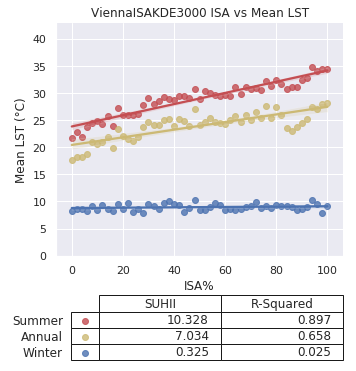
\includegraphics[width=5cm]{ViennaISAKDE3000.png}
\end{figure}

Despite looking like a somewhat reasonable line of fit, the $R^2$ is abysmally low. One way to think about $R^2$ is to see it how much better the model does at fitting the data, compared to a naive model (i.e. a straight line) as a percentage. Thus when there's a lot of variance within a data plot that's very flat, the first order linear model does not do much better than a naive straight line model, thus the really low $R^2$. Despite that, the line fitted is not as horrible as the $R^2$ would suggest. Its usefullness as the central variable in the radius sensitibity test is thus questionable.

\subsection{Bias in Predictions}
Another shortcoming of $R^2$ is its inability to say anything meaningful about any biases in predictions. It is still possible for an invalid model (e.g. a third order relationship modeled as a first ordered one) to produce high $R^2$ values.

\begin{figure}[htb]
    \begin{subfigure}{0.36\textwidth}
        \centering
        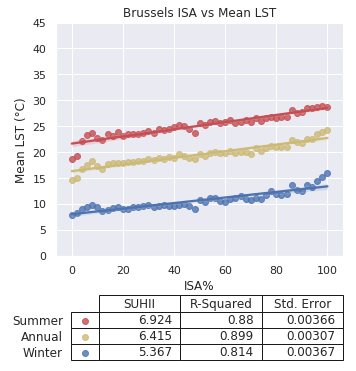
\includegraphics[width=1\linewidth]{Brussels.png}
        \caption{Brussels SUHII at 3000m KDE Radius}
        \label{fig:subim4}
    \end{subfigure}
    \begin{subfigure}{0.6\textwidth}
        \centering
        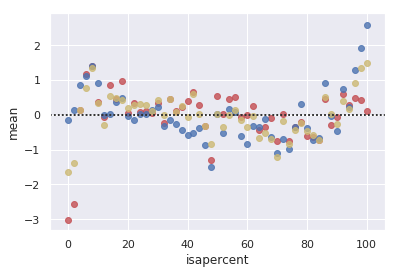
\includegraphics[width=1\linewidth]{BrusselsResid.png}
        \caption{Residual plot of the fitted linear regression}
        \label{fig:subim5}
    \end{subfigure}
    
\end{figure}

Seen above, the analysis using the city of Brussels produced fitted lines with very high $R^2$ values. However, as the residual plot shows, the data deviates from the model in a very regular pattern. Such a residual plot suggests that there's plenty of room for improvement for the model, and indeed, fitting third order polynomial linear regression instead creates much more sensible residual plots.

\begin{figure}[!htb]
    \begin{subfigure}{0.36\textwidth}
        \centering
        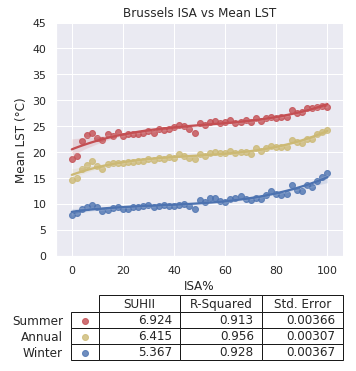
\includegraphics[width=1\linewidth]{Brussels3.png}
        \caption{Brussels SUHII with 3rd order polynomial}
        \label{fig:subim6}
    \end{subfigure}
    \begin{subfigure}{0.6\textwidth}
        \centering
        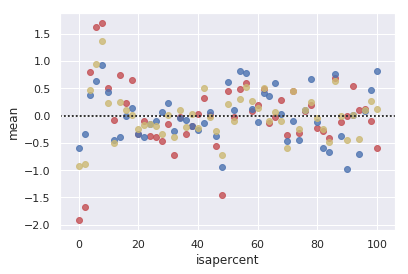
\includegraphics[width=1\linewidth]{Brussels3Resid.png}
        \caption{Residual plot of the fitted polynomial linear regression}
        \label{fig:subim7}
    \end{subfigure}
    
\end{figure}

\subsection{Further Outlook}
None of this analysis invalidates this method's ability to obtain a surface heat island intensity, as the method is still a very reasonable way to produce the difference between urban and non-urban surface temperatures using solely remote sensing satellite data.

However, it is also clear that there is more interesting trends and effects at work. The precise relationship between impervious surface and land surface temperature detected isn't necessarily a clear linear relationship, nor should that be expected. The heterogenous of the urban landscape combined with the radiance effect of all kinds of materials makes the relationship very complicated, with even begining to consider the third dimension that's also a primary driver of the urban landscape.

Despite that, the results we got from the method on a variety of different (primarily European) cities still showed a clear positive trend (also negative in some cases), and that trend deviates from a fitted first order linear line in a clear and consistent way, across KDE radiuses and seasons. The precise underlying mechanics, in terms of both thermodynamics as well as the detection thereof, is not completely understood, but it could provide variable and intriguing information about the urban temperature landscape, as well as its management.

For those reasons, this topic can be further investigated into as a Master's thesis topic. The main points of entry for research are:

\begin{itemize}
    \item Up-to-date research on the Urban Heat Island effect
    \item Basic mechanics of how LST data is derived
    \item The radiance effect used in this particular method
    \item Applicable statistical analyses for these types of data
    \begin{itemize}
        \item i.e. going beyond $R^2$
    \end{itemize}
\end{itemize}



The current expected outcomes are:

\begin{itemize}
    \item Find the most reasonable and applicable kernel radius
    \item Extract more meaningful information from the trend between \%ISA and KDE
    \begin{itemize}
        \item i.e. going beyond the $\Delta T$
        \item Ideally, to be able to classify cities based on their surface thermo-characteristics
    \end{itemize}
    \item Creating a model which can more accurately show the relationship between \%ISA and LST
    
\end{itemize}

\section{Description of Delivered Data}
The shapefiles of the following cities are appended with three additional columns of data named \textit{SummerSUHII}, \textit{WinterSUHII} , and \textit{AnnualSUHII}:
\begin{itemize}
    \item Africa
    \begin{itemize}
        \item Addis Ababa
        \item Casablanca
        \item Johannesburg
        \item Nairobi
        \item Tshwane
    \end{itemize}
    \item Americas
    \begin{itemize}
        \item Chicago
        \item Medellin
        \item Montreal
        \item Pheonix
        \item Portland
        \item Santiago Di Chile
        \item Vancouver
    \end{itemize}
    \item Asia
    \begin{itemize}
        \item Ankara
        \item Beijing
        \item Delhi
        \item Dubai
        \item Hong Kong
        \item Izmir
        \item Jerusalem
        \item Niigata
        \item Seoul
        \item Shizuoka
        \item Singapore
        \item Taipei
        \item Tehran
    \end{itemize}
    \item Australia
    \begin{itemize}
        \item Melbourne
        \item Sydney
    \end{itemize}
    \item Europe
    \begin{itemize}
        \item Amsterdam
        \item Athens
        \item Berlin
        \item Birmingham
        \item Brussels
        \item Budapest
        \item Copenhagen
        \item Dublin
        \item Geneva
        \item Glasgow
        \item Gothenburg
        \item Hamburg
        \item Helsinki
        \item Lisbon
        \item London
        \item Madrid
        \item Milan
        \item Munich
        \item Oslo
        \item Paris
        \item Prague
        \item Rome
        \item Strasburg
        \item Tallinn
        \item Turin
        \item Vienna
        \item Warsaw
        \item Zuerich
    \end{itemize}
\end{itemize}

For code used, raw data produced, and visualizations for cities see:
\textit{https://github.com/wang4918/suhiitest}

\medskip

\printbibliography

\end{document}
